\chapter{手法}

\section{深層学習}

本説では、深層学習の基礎的な用語について述べる。

\subsection{ニューラルネットワーク}

生物の神経回路網を模倣した統計モデルをニューラルネットワークと言い、
多層のニューラルネットワークを利用してモデルを構築する手法を一般に深層学習と呼ぶ。
ニューロンと呼ばれる単純な計算ユニットを多数連結させることでモデルに十分な自由度を持たせ、
複雑な関数を表現することを可能にしている。
入力が入ってくる1層目を入力層、出力を行う最終層を出力層、残りのすべての層を隠れ層と呼ぶ。

各層の全ニューロンが次の層の全ニューロンと結合を持っているニューラルネットワークを全結合ニューラルネットワークという。
\figref{fig:neural_network}に全結合ニューラルネットワークの概略図を示す。
全結合ニューラルネットワークの各層を\term{全結合層}[Fully Connected Layer][Dense Layer]と呼ぶ。
\begin{figure}[tbp]
    \centering
    \includegraphics[width=0.8\columnwidth]{../resource/neural_network.png}
    \caption{全結合ニューラルネットワークの概略図} \label{fig:neural_network}
\end{figure}

ニューラルネットワークには結合の様式によって
\figref{fig:neural_network}に示した全結合ニューラルネットワークのほか、
画像データのモデリングに用いる\term{畳み込みニューラルネットワーク}[Convolution Neural Network]、
系列データのモデリングに用いる\term{再帰的ニューラルネットワーク}[Recurrent Neural Network]などの種類がある。
畳み込みニューラルネットワークの各層を\term{畳み込み層}[Convolution Layer]、再帰的ニューラルネットワークの各層を\term{再帰的層}[Recurrent Layer]とそれぞれ呼ぶ。

\subsection{誤差逆伝播法}

ニューラルネットワークを学習するためには、全ての層が持つパラメータを決定する必要がある。
そこで、\term{確率的最急降下法}[Stochastic Gradient Decent Method, SGD]を用いて最適化を行う。

SGDでは、モデルを評価する損失関数$E$を設定し、各パラメータ$\theta$における勾配$\frac{\partial E}{\partial \theta}$
を求め、$E$を最小化する方向に各パラメータ$\theta$を少しずつ調整する。
勾配$\frac{\partial E}{\partial \theta}$を求める手法として\term{誤差逆伝播法}[Back Propagation] \cite{backpropagation}が存在する。
合成関数の微分における連鎖律を利用することで出力に近い層から順に勾配を計算することが可能である。
\begin{enumerate}
    \item 各層を通してニューラルネットワークの予測値を得る(順伝播)
    \item 予測値と実測値を元に損失関数$E$を計算する
    \item 誤差逆伝播の結果を元に各層のパラメータ$\theta$を調節する
\end{enumerate}

SGDの拡張にあたる最適化手法として、Adagrad\cite{adagrad}やAdam\cite{adam}が存在する。

\subsection{活性化関数}

ニューラルネットワークは複数の層を通して入力と出力との関係をモデリングする。
この際、非線形な関係を学習するために導入するのが活性化関数である。

活性化関数は各層の出力にかける関数で、一般には\figref{fig:activation_function}に示すような
TanhやReLU\cite{relu}、Sigmoid\cite{sigmoid}やSELU\cite{selu}が用いられる。
\begin{figure}[tbp]
    \begin{minipage}[h]{0.49\hsize}
    \centering
    \includegraphics[width=0.9\columnwidth]{../resource/tanh.png} 
    \subcaption{Tanh} \label{fig:tanh}
    \end{minipage}
    \begin{minipage}[h]{0.49\hsize}    
    \centering
    \includegraphics[width=0.9\columnwidth]{../resource/relu.png}
    \subcaption{ReLU} \label{fig:relu}
    \end{minipage}
    \begin{minipage}[h]{0.49\hsize}
    \centering
    \includegraphics[width=0.9\columnwidth]{../resource/sigmoid.png} 
    \subcaption{Sigmoid} \label{fig:sigmoid}
    \end{minipage}
    \begin{minipage}[h]{0.49\hsize}
    \centering
    \includegraphics[width=0.9\columnwidth]{../resource/selu.png}
    \subcaption{SELU} \label{fig:selu}
    \end{minipage}
\caption{種々の活性化関数} \label{fig:activation_function}
\end{figure}

\subsection{多クラス分類への応用}

ニューラルネットワークで多クラス分類を行う場合、出力が各クラスの確率として解釈できる必要がある。
そこで、$N$クラス分類を行う場合は出力層の次元を$N$とし、Softmaxと呼ばれる変換を施す(\eqref{eq:softmax})。
\begin{align}
    y_i = \frac{\exp(x_i)}{\sum_{j=1}^N \exp(x_j)} \label{eq:softmax}
\end{align}

$x_i$は$[-\infty, \infty]$を取るが、$\exp$をかけることで全ての出力を正にすることができる。
その後、全クラスの出力の合計値を$1$にするように正規化を行うことで、各クラスの出力は確率として解釈できるようになる。

\section{深層生成モデル}

データ$x$と、そのデータが所属するクラスを表すラベル$y$から分類境界を直接モデリングし、クラス分類を行う手法を判別モデルという。
判別モデルとしては\term{Support Vector Machine}[SVM]や\term{Random Forest Classification}など、
多くの手法が提案されている。
データ$x$と実測値$y$から回帰曲面を直接モデリングし、回帰を行う手法を回帰モデルという。
回帰モデルには\term{Support Vector Regression}[SVR]や\term{Random Forest Regression}などが含まれる。

一方、生成モデルではデータ$x$が潜在変数$z$から生成されたと考える。
そして、潜在変数の分布$p(z)$とデータの分布$p(x)$との変換規則$p(x|z)$をモデリングする。
潜在変数の分布$p(z)$からサンプリングして生成モデルに通すと、$p(x)$、
すなわちデータの分布に沿ってサンプルを生成することができる。

深層学習を利用しない生成モデルとしては、\term{Gaussian Mixture Model}[GMM]や
\term{Hidden Markov Model}[HMM]、\term{Latent Dirichlet Allocation}[LDA]などが存在する。

生成モデルに深層学習を用いた手法を深層生成モデルという。
代表的な深層生成モデルとしては
\begin{itemize}
    \item Variational Autoencoders (VAE)
    \item Generative Adversarial Networks (GAN)
    \item Adversarial Autoencoders (AAE)
\end{itemize}
などが挙げられる。

\subsection{Variational Autoencoders (VAE)} \label{vae}

\figref{fig:vae}に\term{Variational Autoencoders}[VAE]\cite{Kingma2014, Doersch2016}の概略図を示す。
VAEとは、潜在変数に正規分布$\mathcal{N}(0, 1)$を仮定したAutoencodersの一種である。
\begin{figure}[tbp]
    \centering
    \includegraphics[width=0.8\columnwidth]{../resource/vae.png}
    \caption{VAEの概略図} \label{fig:vae}
\end{figure}

入力$x$から潜在変数$z$への変換を行うEncoderと$z$から$x$への変換を行うDecoderを同時に学習させる。
すなわち、$p(z|x)$をEncoderモデル$\Enc(z|x)$で、$p(x|z)$をDecoderモデル$\Dec(x|z)$で近似させる。

$\Enc(z|x)$の学習とは$\Enc(z|x)$と$p(z|x)$のKullback-Leibler divergenceを最小にすることであるから、
\begin{align*}
    \KL[\Enc(z|x)||p(z|x)] &= \E[\log \Enc(z|x) - \log p(z|x)]\\
    &= \E[\log \Enc(z|x) - \log p(x|z) - \log p(z)] + \log p(x)\\
    &= \KL[\Enc(z|x)||p(z)] - \E[\log p(x|z)] + \log p(x)
\end{align*}
より、
\begin{align}
    \KL[\Enc(z|x)||p(z|x)] - \log p(x) = \KL[\Enc(z|x)||p(z)] - \E[\log p(x|z)] \label{eq:vae_loss}
\end{align}
が成り立つ。左辺第1項を最小化することはEncoderを学習することを表し、
左辺第2項を最小化することはAutoencoders全体を学習することを意味する。

よって、\eqref{eq:vae_loss}の右辺がVAEにおける損失関数(Loss)となり、これを最小化することが学習の目的である。

\subsubsection{ネットワークの構成法}

Encoderは適当なニューラルネットワークで作成するが、その出力$z$は正規分布$\mathcal{N}$に従うと仮定する。
この仮定に基づくと、Encoderは平均$\mu(x)$と分散$\Sigma(x)$を出力するネットワークとして設計することができる。

Decoderは$\mu(x)$と$\Sigma(x)$から1点をサンプリングし、そこから$x$を再構成するネットワークとして設計すれば良い。

\subsubsection{Reparametrization Trick} \label{reparametrization_trick}

\eqref{eq:vae_loss}において、$\E[\log p(x|z)]$を計算するためにはサンプリングが用いられる。
しかし、ニューラルネットワーク中でサンプリングを行ってしまうと計算グラフが途切れてしまうため、誤差逆伝播法による学習を行うことができない。
そこで用いられるのがReparametrization Trickと呼ばれる手法である。

$\mathcal{N}(\mu, \Sigma)$からサンプリングする代わりに
$e\sim \mathcal{N}(0, 1)$として$z = \mu(x) + e\Sigma(x)$を計算する。
このように計算を行うことで、サンプリングと等価な演算を行いながら誤差逆伝播法による学習も行うことが可能になる。

\subsubsection{Conditional VAE (CVAE)への拡張}

VAEの拡張として、潜在変数の生成に目的変数の情報を考慮できるConditional VAE(CVAE)\cite{Kingma2014}が提案されている。
KingmaらはCVAEを用いたM1+M2モデルという深層生成モデルを提案した。
M1+M2モデルは目的変数の情報を考慮しないM1モデルを予め大量の教師なしのデータで学習させておき、
得られた潜在変数を用いて目的変数の情報を考慮するM2モデルを僅かな教師付きデータと大量の教師なしデータを混ぜて学習するモデルである。
このモデルは手書き文字認識タスクMNISTにおいて、70,000枚中わずか100枚にのみ正解を与える半教師付き学習で正解率96\%を達成した。
このように、CVAEは半教師付き学習のフレームワークとして利用可能である。

\subsection{Generative Adversarial Networks (GAN)} \label{gan}

\figref{fig:gan}に\term{Generative Adversarial Networks}[GAN] \cite{gan}の概念図を示す。
GANとは、GeneratorとDiscriminatorという2つのモデルを敵対的に学習させることによってデータを生成させる枠組みである。
Generator $G(z)$は乱数$z$から実データと似たデータ$G(z)$を生成する。Discriminator $D(x)$は実データとGeneratorが作り出したデータを判別する。
\begin{figure}[tbp]
    \centering
    \includegraphics[width=0.8\columnwidth]{../resource/gan}
    \caption{GANの概念図} \label{fig:gan}
\end{figure}

GANで用いられる目的関数は以下の式で表される。
\begin{align}
    \min_{G}\max_{D}V(D, G) = \E_{x\sim p_{\data}(x)}[\log D(x)] + \E_{z\sim p_{z}(z)}[\log(1-D(G(z)))] \label{eq:gan_loss}
\end{align}
Discriminatorを学習する際はGeneratorを固定した上で\eqref{eq:gan_loss}を最大化する。
右辺第1項は実際のデータに対応した項で、この項を最大化するためには実データに対してDicriminatorが$1$と判断すれば良い。
右辺第2項はGeneratorが生成したデータに対応した項で、この項を最大化するためにはGeneratorが生成したデータに対して$0$と出力すればよい。

Generatorを学習する際はDiscriminatorを固定した上で\eqref{eq:gan_loss}を最小化すればよい。
第1項はGeneratorに依存しないので第2項のみを考える。
第2項を最小化するためには$D(G(z))$を1に近づける、すなわち、Generatorが生成した画像に$1$というラベルをつけて学習させればよい。

\subsection{Adversarial Autoencoders (AAE)} \label{aae}

Adversarial Autoencoders (AAE) \cite{aae}とは、オートエンコーダに対してGANの枠組みで正則化を行う手法である。

VAEではKullback-Leibler divergenceを解析的に計算するために潜在変数を単純な正規分布と仮定する必要があったが、
AAEではGANの枠組みで正則化を行うことで潜在変数を任意の分布に近づけることができる。

\subsubsection{AAEの概要}

\figref{fig:adv_ae}にAAEの概略図を示す。
AAEは基本的にはオートエンコーダであるため、入力$x$を潜在変数$z$にエンコードしたり、
$z$を$x$にデコードしたりする。
オートエンコーダにおけるEncoderをGenerator $G$として扱う。
Discriminator $D$はオートエンコーダとは別のネットワークとして定義し、
与えられた$z$がGeneratorを通した後の$q(z)$由来のものなのか、任意の分布$p_z(z)$からサンプリングしたものなのかを判別する。
\begin{figure}[tbp]
    \centering
    \includegraphics[width=0.8\columnwidth]{../resource/adv_ae.pdf}
    \caption{Adversarial Autoencodersの概略図\cite{aae}} \label{fig:adv_ae}
\end{figure}

目的関数は\eqref{eq:gan_loss}と類似しており、
\begin{align}
    \min_{G}\max_{D}V(D, G) = \E_{z\sim p_z(z)}[\log D(z)] + \E_{x\sim p_{\data}(x)}[\log(1-D(G(x)))] \label{eq:aae_loss}
\end{align}
で表される。任意の分布$p_z$からサンプリングしたものを真のデータと見なしている点と、
GANとは$x$と$z$が逆になっている点に注意が必要である。

学習の際は、
\begin{enumerate}
    \item オートエンコーダ部分を復元誤差を最小化するように学習させる
    \item Discriminatorを\eqref{eq:aae_loss}を最大化するように学習させる
    \item Generatorを\eqref{eq:aae_loss}を最小化するように学習させる
\end{enumerate}
の順で行う。

\eqref{eq:aae_loss}を最小化するためには$\log(1-D(G(x)))$を最小化すればよく、
$D(G(x))$を$1$に近づければ良い。これは、Generatorの生成結果をDiscriminatorが真のデータと予測することを意味する。
したがって、Generatorを学習させる過程で、潜在変数$q(z)$を$p(z)$に近づけることができる。

\subsubsection{AAEの半教師付き学習への応用}

AAEを半教師付き学習に応用する場合のアーキテクチャを\figref{fig:adv_ae_semi}に示す。
Disciriminatorにクラスを表すラベルを入力することで、Discriminatorがラベルの情報を使って分類することが可能になる。
ラベルを参照するDiscriminatorを騙すため、Generatorは同じラベルを持ったサンプルを近づけるように学習するようになる。
\begin{figure}[tbp]
    \centering
    \includegraphics[width=0.75\columnwidth]{../resource/adv_ae_semi.pdf}
    \caption{AAEを半教師付き学習へ応用する場合の構造\cite{aae}} \label{fig:adv_ae_semi}
\end{figure}

Discriminatorに与えるラベルに「ラベルなし」というクラスを用意することで、AAEを半教師付き学習として利用することができる。
本研究では、このアーキテクチャを利用した。

\subsection{Positive-Unlabeled GAN (PUGAN)} \label{pugan}

Positive-Unlabeled GAN (PUGAN) \cite{pugan}とは、GANにpositive-unlabeled learningの枠組みを組み合わせた手法である。
positive-unlabeled learning自体は古くから存在する考え方で、僅かな正例と大量のラベルなしデータを利用して機械学習を行うという発想である。

\figref{fig:gpu_scheme}にPUGANの概念図を示す。PUGANは3つのDiscriminatorと2つのGeneratorを持つ。
それぞれの役割は以下の通りである。
\begin{itemize}
    \item Positive Generator: 正例らしいデータを生成する
    \item Negative Generator: 負例らしいデータを生成する
    \item Positive Discriminator: 正例とPositive Generatorが生成した正例を判別する
    \item Unlabeled Discriminator: ラベルなしデータとGeneratorが生成したデータを判別する
    \item Negative Discriminator: 正例とNegative Generatorが生成した負例を判別する
\end{itemize}
特徴的なのは正例である$x_p$を2回入力として用いる点である。
\begin{figure}[tbp]
    \centering
    \includegraphics[width=0.8\columnwidth]{../resource/gpu_scheme.jpg}
    \caption{PUGANの概略図\cite{pugan}} \label{fig:gpu_scheme}
\end{figure}

生成を行う際はPositive Generatorに乱数を入力することで正例らしいデータを生成することができる。

\section{深層学習で文字列を扱う手法}

\subsection{文字列の埋め込み(Embedding)} \label{embedding}

文字列はそのままニューラルネットワークの入力にすることはできない。
そこで、文字列の各要素を多次元の数値ベクトルに変換する必要がある。これを\term{埋め込み}[Embedding]という。
一般的な文章の場合は各単語を、SMILESの場合は各文字を、それぞれ埋め込むことになる。

方法のひとつは\figref{fig:onehot}に示すOne-Hot Encodingである。
SMILESに含まれる文字種を抽出した後、その各文字に対して該当する文字種のビットだけが1になっているダミー変数に変換する。
データセットに含まれる文字種が$M$種類、SMILESの長さが$N$文字であった場合、ひとつの構造は$M\times N$の行列で表す。
実際には分子によってSMILESの長さが異なるため、データセット中で最も長いSMILESを持つ分子の長さを$N$に設定し、
足りない部分はすべて空白埋めを行って長さを揃える。
One-Hot Encodeされたベクトルは文字列と1対1対応するため、モデルの出力としてOne-Hot Encodeされたベクトルを得られれば直にSMILES文字列を得たことに相当する。
\begin{figure}[tbp]
    \centering
    \includegraphics[width=0.8\columnwidth]{../resource/onehot.png}
    \caption{One-Hot Encodingの概念図} \label{fig:onehot}
\end{figure}

もうひとつの方法は多くのニューラルネットワークライブラリに実装されているEmbeeding Layerを用いる方法である。
One-Hot Encodingが多くの0を含むスパースな埋め込みになるのに対し、
Embedding Layerを用いた場合は非零要素が少ない密ベクトルでの埋め込みとなる。
埋め込み方はEmbedding Layerをランダムに初期化した後、誤差逆伝播法によってモデルと同時に学習させる。
Embedding Layerを用いた場合も、モデルの出力としてはOne-Hot Encodeされたベクトルを得ることを目指す。

本研究ではいずれの埋め込み方法も試し、性能の優劣を確認した。

\subsection{Recurrent Neural Network (RNN)}

系列データを扱うための深層学習モデルを総称して\term{Recurrent Neural Network}[RNN]と言う。
RNNは内部状態を持っており、系列を順番に読み込み、内部状態をアップデートしながら予測を行う。

層の出力と入力を単純に接続し、前回の出力を考慮した計算を可能としたものを単純RNN\cite{simple_rnn}と呼ぶ。
単純RNNは考慮するステップが多くなった場合に勾配消失や勾配爆発が起こるという問題があった。
勾配消失や勾配爆発が起こると誤差逆伝播法による学習を行うことができない。
そこで、\term{Long Short-Term Memory}[LSTM] \cite{lstm_original, lstm_forget_gate, lstm_peephole}と
\term{Gated Recurrent Unit}[GRU] \cite{gru}が提案されている。

LSTMは何度かのアップデートを経て性能が向上した手法である。
HochreiterらはLSTMに状態を記憶するメモリセルを用意し、
メモリセルを書き換えるべきかを判断する入力ゲートとメモリセルの内容を出力すべきか判断する出力ゲートを提案した\cite{lstm_original}。
Gersらは系列の傾向が大きく変わった際に以前の情報を適切に忘れるために忘却ゲートを提案した\cite{lstm_forget_gate}。
Gersらは各ゲートの判断が系列のみに依存していることに着目し、メモリセル自体がゲートの判断に関与することを可能にするPeephole Connectionを提案した\cite{lstm_peephole}。
他にもいくつかの改善が存在するが、多くのライブラリに実装されているLSTMはここまでの改善を反映したものである。

ChoらはLSTMの構造が複雑であることに注目し、ゲートを更新ゲートとリセットゲート2つに絞ったGRUを提案した\cite{gru}。
GRUはパラメータが少ないこともあり、特にデータ数が少ない状況で効果を発揮する。

本研究ではLSTMとGRUについて比較を行った。

\subsection{Teacher Forcing} \label{teacher_forcing}

文字列を生成させるモデルの場合、先頭から順次生成させるのが一般的である。
\figref{fig:sequence_generation}に文字列生成の概略を示す。
最初は開始トークンを入力して各文字の確率を出力として得た後、確率最大の文字を1文字目とする。
2文字目以降は以前の出力を入力とする。以前の文字から次の文字を予測することになるため、
文字列の後半になると誤差が蓄積され、学習が不安定になったり意味のある文字列が生成されなくなるという問題がある。
\begin{figure}[tbp]
    \centering
    \includegraphics[width=0.8\columnwidth]{../resource/sequence_generation.png}
    \caption{文字列生成の概略図} \label{fig:sequence_generation}
\end{figure}


この問題に対処するため提案されたのがTeacher Forcing\cite{teacher-forcing}である。
\figref{fig:teacher_forcing}にTeacher Forcingの概略を示す。
Teacher Forcingを適用する場合、訓練時は予測された文字ではなく、正解の文字を次への入力とする。
これにより学習が安定し、収束が早くなるメリットがある。
\begin{figure}[tbp]
    \centering
    \includegraphics[width=0.8\columnwidth]{../resource/teacher_forcing.png}
    \caption{Teacher Forcingの概略図} \label{fig:teacher_forcing}
\end{figure}


Teacher Forcingのデメリットとしては、推論時には学習時と異なる状況で推論を行わなければいけないという点が挙げられる。
この問題を改善するために、Scheduled Sampling\cite{scheduled-sampling}が提案されている。
\figref{fig:scheduled_sampling}にScheduled Samplingの概略を示す。
Scheduled Samplingを利用する場合、正解の文字を確率$p$で、予測された文字を確率$1-p$でサンプリングして次の入力とする。
\begin{figure}[tbp]
    \centering
    \includegraphics[width=0.8\columnwidth]{../resource/scheduled_sampling.png}
    \caption{Scheduled Samplingの概略図} \label{fig:scheduled_sampling}
\end{figure}


Scheduled Samplingの確率を$p=0$とした場合は通常の学習、$p=1$とした場合はTeacher Forcingとなる。
一般にはScheduled Samplingも含めてTeacher Forcingと呼ぶため、本研究でもそれに倣った。

\subsection{Convolutional Neural Network (CNN)} \label{cnn}

\term{Convolutional Neural Network}[CNN][畳み込みニューラルネットワーク] とは、一般に画像解析の際に用いられる深層学習手法である。
CNNは複数のフィルタを局所的にかけていくことで画像から特徴を抽出する。

近年、CNNは文字列解析にも用いられるようになっている。
画像解析で用いられるCNNはフィルタが2次元であるが、文字列解析では1次元のフィルタを用いる。
1次元のフィルタを用いたCNNをConv1Dと表記することが多い。

CNNに特有のパラメータとして、カーネルサイズとフィルタ数がある。
カーネルサイズはどの程度近傍の情報を利用するかというパラメータで、
大きくするほど全体的な特徴を、小さくするほど局所的な特徴を取得するようになる。
フィルタ数は近傍のとり方の種類数を表す。

\section{深層生成モデルを化学データに適用した先行研究}

本節では、深層生成モデルを化学データに適用した先行研究について概説する。

\subsection{化合物から連続的な潜在表現を取り出す}

G\'{o}mez-Bombarelliらは\term{Variational Autoencoder}[VAE]を用いて、
化学構造の線形表記の1種であるSMILESから連続値の潜在表現を得る手法を提案した\cite{Gomez-Bombarelli2016}。
これをchemical VAEと呼ぶ。

\figref{fig:chemical_vae}にchemical VAEの概念図を示す。
chemical VAEは化学構造のSMILES表記を入力とし、SMILES表記から連続潜在変数を取り出すエンコーダと
潜在変数からSMILES表記を復元するデコーダを用意し学習を行う。
エンコーダには文字列を畳み込む1次元CNNを、デコーダには文字列を生成するRNNを用いることが多い。
潜在変数空間中の1点を指定してデコーダに通すことで、対応するSMILESを直に得ることができる。
\begin{figure}[tbp]
    \centering
    \includegraphics[width=0.8\columnwidth]{../resource/chemical_vae.png}
    \caption{chemical VAEの概念図} \label{fig:chemical_vae}
\end{figure}

所望の活性値を持つ化学構造を得る場合、2通りのアプローチが存在する。
1つは学習した潜在変数を特徴量とし、活性値との間で新たな統計モデルを構築する手法である。
もう1つは学習したchemical VAEは構造の組み立てにのみ用い、活性値の予測は通常のQSPRと同様に記述子を計算して行うという手法である。
いずれの場合でも、活性値との関係を学習するためには多量のデータが必要になるという問題点が存在する。

\subsection{種々の深層生成モデルを比較する}

Blaschkeらは複数の深層生成モデルを比較し、
AAEとベイズ最適化を組み合わせることで医薬品である確率が高く、新規な構造を生成できることを示している\cite{Blaschke2018}。

用いているデータセットはEsCAPE-DBから抽出した\term{Dopamine Receptor D2}[DRD2]データセットである。
検証の流れはChEMBL22でVAE、AAEの各モデルを学習した後、得られた潜在変数空間と活性値との間で
\term{Support Vector Machine}[SVM]を用いた活性予測モデルを構築する。
その後活性予測モデルの出力を最大化するように潜在変数空間中でベイズ最適化を行う。

しかし、DRD2は正例$7,218$件、負例$343,204$が存在する比較的大きなデータセットである。
データセットが小さくなった場合、ベイズ最適化の目的関数となる活性予測モデルの外挿能力が低下するという問題が発生する。
目的関数が信頼できない状況で行ったベイズ最適化の結果は同様に信頼することが難しい。
AAEの潜在変数には活性の情報が反映されていないため、AAEの潜在変数から直接サンプリングを行って新規構造を生成することも困難である。

\section{提案手法}

本研究では、以下の3つの手法を半教師付き学習的に化学データに適用し、検証を行った。
\begin{itemize}
    \item Variational Autoencoders (VAE) \cite{Kingma2014, Doersch2016}
    \item Adversarial Autoencoders (AAE) \cite{aae}
    \item Positive-Unlabeled GAN (PUGAN) \cite{pugan}
\end{itemize}
本節では各手法を適用した場合について詳説する。

\subsection{VAEを用いた高精度な活性予測}

\figref{fig:vae_prediction_model}に提案手法の概念図を示す。
M1モデルでは活性値の情報のついていない大量の化学構造データから、SMILESと化学構造一般の特徴(潜在変数①)の対応付けを学習する。
M2モデルではわずかな活性値付きデータを混ぜて学習し、化学構造一般の特徴(潜在変数①)と活性値との関係を潜在変数②に落とし込む。
\begin{figure}[tbp]
    \centering
    \includegraphics[width=0.8\columnwidth]{../resource/vae/scheme.png}
    \caption{VAEを利用した半教師付き学習} \label{fig:vae_prediction_model}
\end{figure}

デコーダ②に活性値を通した場合、潜在変数②の情報と活性値の両方から最も尤もらしいSMILESを組み立てる構造生成器として利用する。
デコーダ②に活性値を通さなかった場合、潜在変数②から活性値を予測する予測モデルとしても使用可能になるような設計を検討した。
活性値のついていないデータはChEMBL\cite{chembl22}やZINC\cite{zinc12, zinc15}などのデータベースから容易に取得可能であり、今回はChEMBLを利用した。
実験化学者が各々で取得している少量の活性データなどと組み合わせて良好な予測・構造生成を行うことを目指した。

\subsection{AAEを用いた構造提案}

大量のデータを利用した場合、AAEで良好な構造提案ができることはBlaschkeらの研究\cite{Blaschke2018}によって示されている。
そこで、本研究の着眼点は少数データにおいてAAEが適用できるか確認することにある。

\figref{fig:aae_architecture}にAAEを適用する場合の概略図を示す。
本研究では入力$x$に化学構造の線形表記であるSMILESを利用し、SMILESを2次元のガウス分布に変換することを目指した。
半教師付き学習を行うため、Discriminatorに与えられた構造が活性値情報を持っているか否かの情報を与えた。
EncoderはDecoderで正しく構造が復元できること、
およびDiscriminatorを誤分類させることを目指して学習を行った。
このように学習を行うことで潜在変数$z$が上で挙げた望ましい性質を満たすようになった。
\begin{figure}[tbp]
    \centering
    \includegraphics[width=0.95\columnwidth]{../resource/aae/architecture.png}
    \caption{AAEを適用する場合の概略図} \label{fig:aae_architecture}
\end{figure}

\subsection{PUGANを用いた構造提案}

\figref{fig:pugan_architecture}にPUGANを適用する場合の概略図を示す。
本研究では活性ありのデータセットとしてADRA2データセットを、活性値情報なしのデータセットとしてChEMBL22データセットをそれぞれ利用した。
Positive GeneratorとNegative Generatorの入力には一様乱数を利用した。
\begin{figure}[tbp]
    \centering
    \includegraphics[width=0.95\columnwidth]{../resource/pugan/architecture.png}
    \caption{PUGANを適用する場合の概略図} \label{fig:pugan_architecture}
\end{figure}

構造生成を行う場合は、Positive Generatorに一様乱数を与えることでサンプリングを行うことができる。
